% Template LaTeX - Pôster IX Simpósio de Iniciação Científica / UNIFEI
% Dimensões e tipografia ajustadas ao modelo PPTX oficial.
% Versão modular compatível com pdfLaTeX.

\documentclass[portrait]{a0poster}

\usepackage[T1]{fontenc}
\usepackage[utf8]{inputenc}
\usepackage[portuguese]{babel}
% Bera Sans family supplied by the TeX distribution.
\usepackage[scaled]{berasans}
\renewcommand{\familydefault}{\sfdefault}
\usepackage[paperwidth=90cm, paperheight=120cm, left=6.7cm, right=6.7cm, top=15.5cm, bottom=11.5cm]{geometry}

\usepackage{indentfirst}
\usepackage{graphicx}
\graphicspath{{figures/}{./}}
\usepackage{eso-pic}
\usepackage{xcolor}
\usepackage{ragged2e}
\usepackage{multicol}
\usepackage{titlesec}
\usepackage{microtype}
\usepackage{caption}
\usepackage{url}
\usepackage{enumitem}

% ------------------------------------------------------------
% FONTES -- versão compatível com pdfLaTeX
% ------------------------------------------------------------
\newcommand{\posterbody}{\fontfamily{fvs}\selectfont}
\newcommand{\posterheading}{\fontfamily{fvs}\selectfont}

% ------------------------------------------------------------
% CABEÇALHO E RODAPÉ OFICIAIS UNIFEI
% ------------------------------------------------------------
\AddToShipoutPictureBG{%
  \AtPageUpperLeft{%
    \raisebox{-12.25cm}{
\includegraphics[width=\paperwidth]{image2.png}}%
  }%
}
\AddToShipoutPictureBG{%
  \AtPageLowerLeft{%
    \raisebox{-0.15cm}{
\includegraphics[width=\paperwidth]{image3.png}}%
  }%
}

% ------------------------------------------------------------
% PARÂMETROS GERAIS DO PÔSTER
% ------------------------------------------------------------
\pagestyle{empty}
\setlength{\parskip}{0.25em}
\setlength{\emergencystretch}{2em}

\setlength{\columnsep}{4.2cm}
\setlength{\columnseprule}{0pt}

% Corpo: Arial/Bera Sans 23 pt, entrelinha 30 pt, justificado.
\newcommand{\postertext}{%
  \posterbody
  \fontsize{23}{30}\selectfont
  \justifying
  \setlength{\parindent}{1.6cm}%
}

% Títulos das seções: Verdana/Bera Sans 38 pt, negrito.
\newcommand{\sectiontitle}[1]{%
  \scalebox{1.06}[1.02]{%
    \posterheading
    \fontsize{38}{44}\selectfont
    \bfseries
    #1%
  }%
}

\titleformat{\section}
  {\normalfont}
  {}{0pt}{\sectiontitle}

\captionsetup{
  font={small,sf},
  labelfont=bf,
  justification=centering,
  skip=5pt
}

% ------------------------------------------------------------
% COMANDOS PARA TÍTULO/AUTORES
% ------------------------------------------------------------
\newcommand{\postertitle}[1]{%
  \begin{center}
    \parbox{68cm}{%
      \centering
      \posterheading
      \fontsize{60}{70}\selectfont
      \bfseries
      \MakeUppercase{#1}\par
    }%
  \end{center}
}

\newcommand{\posterauthors}[1]{%
  \begin{center}
    {\posterheading\fontsize{34}{38}\selectfont\bfseries\itshape #1\par}
  \end{center}
}

\newcommand{\posterinstitution}[1]{%
  \begin{center}
    {\posterheading\fontsize{34}{38}\selectfont #1\par}
  \end{center}
}

\begin{document}

% ------------------------------------------------------------
% BLOCO SUPERIOR
% ------------------------------------------------------------
\vspace*{-1.75cm}

\postertitle{INTELIGÊNCIA GEOESPACIAL EM TEMPO REAL PARA MITIGAÇÃO DE DESASTRES AMBIENTAIS}

\vspace{0.70cm}

\posterauthors{Gabriel Gonçalves Sampaio, Barbara Pimenta Caetano}

\vspace{-0.90cm}

\posterinstitution{INSTITUTO DE ENGENHARIA DE SISTEMAS E TECNOLOGIA DA INFORMAÇÃO -- UNIFEI}

\vspace{0.70cm}

% ------------------------------------------------------------
% DUAS COLUNAS MODULARES BALANCEADAS
% ------------------------------------------------------------
\begin{multicols}{2}
\postertext

\section*{INTRODUÇÃO}

No monitoramento de incêndios florestais, o registro pontual de uma anomalia térmica apresenta utilidade limitada para a tomada de decisão quando desprovido de contexto espacial e temporal imediato. Para subsidiar ações de campo, a literatura postula a necessidade de construir \textit{Consciência Situacional} (ENDSLEY, 1995) --- a capacidade de perceber, compreender e projetar o efeito de eventos dinâmicos sobre comunidades e infraestruturas do território. Embora o país conte com dados de sensoriamento remoto (INPE, 2026), as informações sobre infraestruturas e vulnerabilidades permanecem distribuídas em bases setoriais descentralizadas (ONS, DATASUS, DNIT, FUNAI), dificultando cruzamentos em tempo hábil.

Diante desse cenário, este projeto avalia o desenvolvimento de uma plataforma analítica geoespacial orientada a eventos. A proposta concentra-se em correlacionar anomalias térmicas e dados de infraestrutura crítica em tempo quase real, buscando prover suporte informacional contínuo para a Defesa Civil e operadores setoriais.

\vspace{0.20cm}
\section*{METODOLOGIA}

O pipeline analítico inicia-se pelo saneamento contínuo dos dados brutos do INPE, aplicando validações de esquema, descarte de leituras duplicadas e eliminação de inconsistências na telemetria satelital. Para reduzir o tempo de processamento espacial em comparação a bancos relacionais convencionais, o cálculo de distâncias relativas às malhas territoriais (rodovias do DNIT, hospitais do CNES, terras da FUNAI e municípios do IBGE) é antecipado diretamente em memória durante a etapa de ingestão.

Para estruturar os dados pontuais, empregam-se algoritmos espaciais específicos: o \textbf{\textit{DBSCAN}} agrupa focos contíguos no espaço e no tempo para delimitar perímetros de queima, enquanto grafos no \textbf{\textit{NetworkX}} representam a malha elétrica do SIN (ONS), estimando o risco de desligamentos e falhas em cascata em linhas e subestações.

\begin{center}
    \vspace{-0.10cm}
    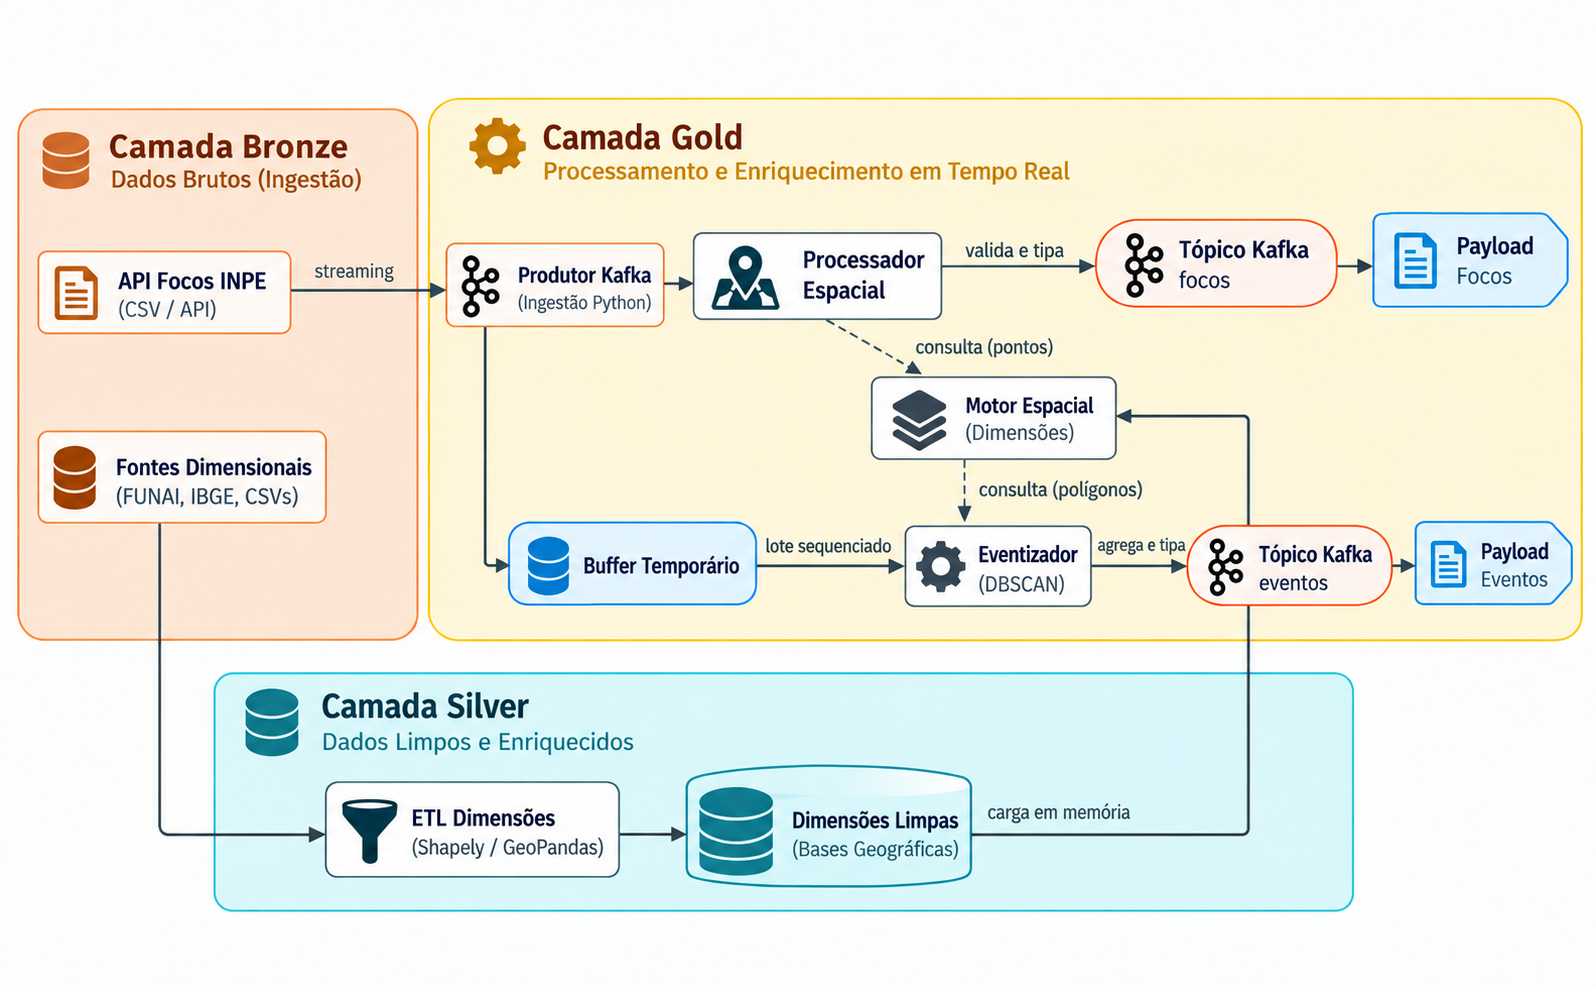
\includegraphics[width=0.55\linewidth]{fig_pipeline_camadas.png}
    \captionof{figure}{Pipeline de ingestão e processamento espacial em memória.}
    \vspace{-0.10cm}
\end{center}

Os eventos enriquecidos alimentam o \textbf{\textit{Apache Kafka}}, que organiza o fluxo de dados entre o registro individual de focos e o encaminhamento de polígonos agregados para a camada analítica.

Na etapa de armazenamento, as mensagens são consumidas pelo banco colunar distribuído \textbf{\textit{Apache Druid}} (YANG et al., 2014). O modelo dimensional adota identificadores numéricos e tabelas de consulta rápida em memória, viabilizando agregações geográficas com menor tempo de resposta (Fig. 2).

\begin{center}
    \vspace{-0.10cm}
    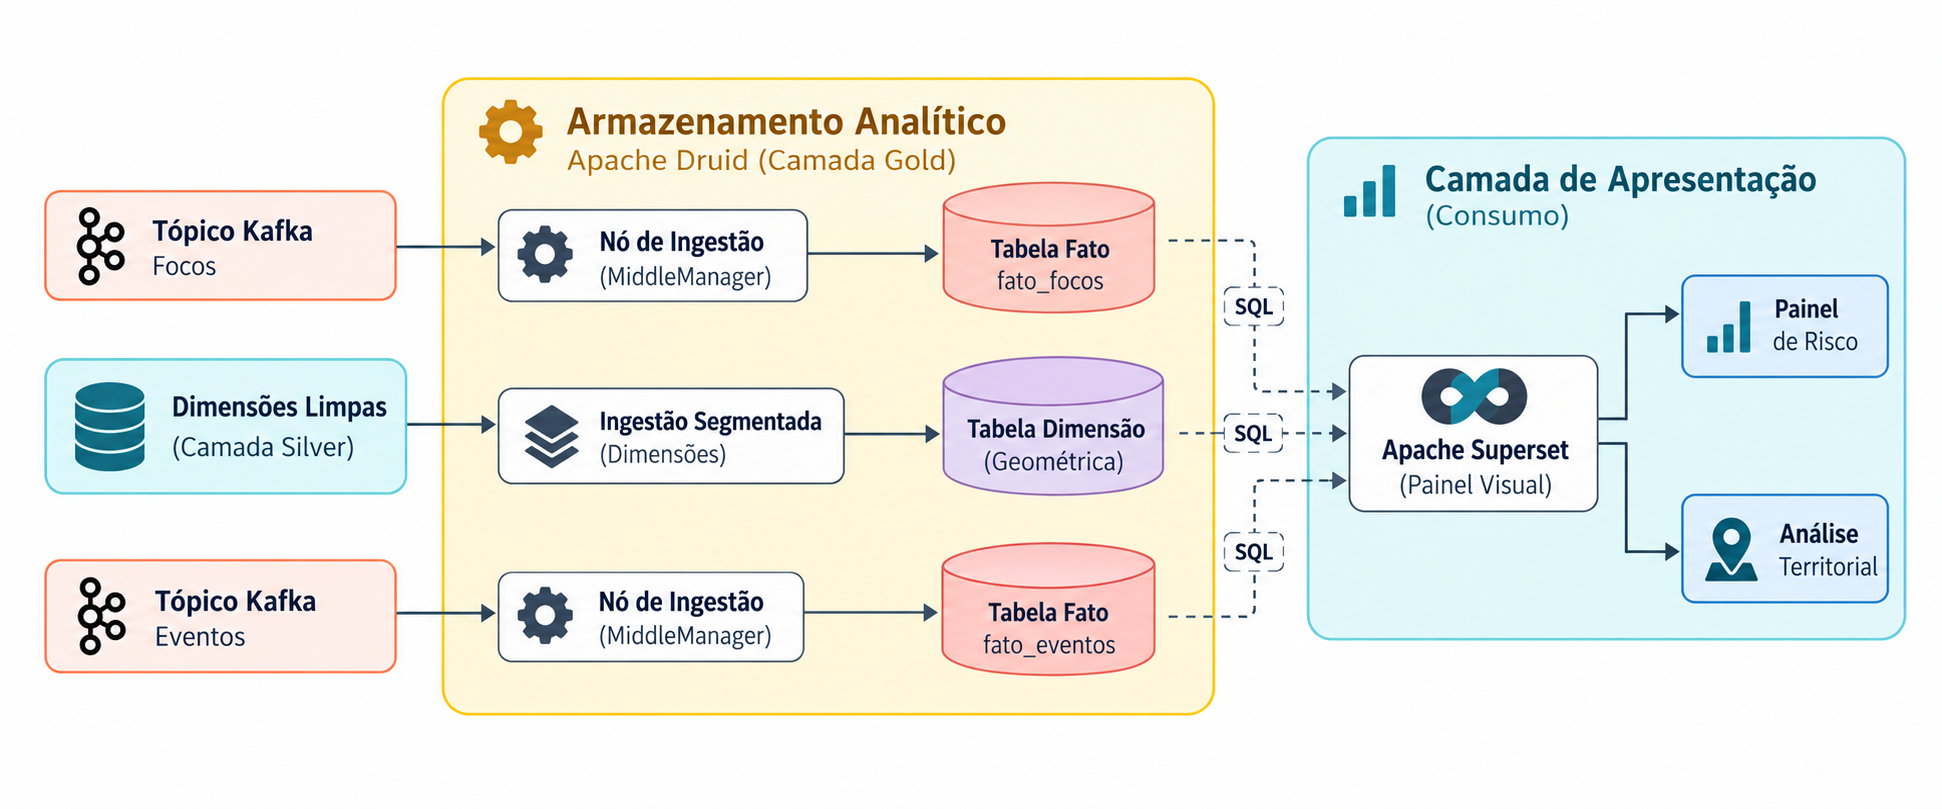
\includegraphics[width=0.55\linewidth]{fig_druid_superset.png}
    \captionof{figure}{Arquitetura analítica com Apache Druid e Apache Superset.}
    \vspace{-0.10cm}
\end{center}

A camada de visualização no \textbf{\textit{Apache Superset}} organiza as métricas em painéis temáticos (visão geral, saúde, terras indígenas e energia), estruturando os dados para suporte à tomada de decisão operacional.

\vspace{0.20cm}
\section*{RESULTADOS E DISCUSSÕES}

A avaliação em escala nacional ao longo do ano de 2025 integrou 4,05 milhões de registros provenientes de 7 bases governamentais, alocados em $\sim$850 MB no \textbf{\textit{Apache Druid}} em 695 segmentos compactados.

\begin{center}
\vspace{-0.10cm}
{\fontsize{16}{20}\selectfont
\begin{tabular}{llr}
\hline
\textbf{Entidade Lógica} & \textbf{Fonte Governamental} & \textbf{Registros Aprox.} \\
\hline
Fato Focos de Incêndio & INPE (BDQueimadas) & 3.335.198 \\
Fato Eventos Agrupados & Algoritmo \textbf{\textit{DBSCAN}} (Perímetros) & 147.560 \\
Hospitais e Unidades de Saúde & MS / DATASUS (CNES) & 550.882 \\
Rodovias Federais e Estaduais & MT / DNIT / BIT & 14.255 \\
Linhas e Subestações de Energia & MME / ANEEL / ONS & 2.564 \\
Municípios Brasileiros & IBGE (Malha Geodados) & 5.564 \\
Terras Indígenas Demarcadas & MJSP / FUNAI & 650 \\
\hline
\textbf{Total Analítico Consolidado} & \textbf{Armazenamento nos Nós Druid} & \textbf{4.056.673 ($\sim$850 MB)} \\
\hline
\end{tabular}
}
\vspace{0.08cm}
\captionof{table}{Volumetria das bases governamentais integradas no território brasileiro.}
\label{tab:volumetria}
\end{center}

\vfill\null\columnbreak

A avaliação de desempenho submeteu o sistema a 29 consultas SQL analíticas em três topologias com restrição de processamento (1,0 vCPU \textit{Baseline}, 1,5 vCPU \textit{Balanced} e 2,0 vCPU \textit{Query Heavy}), variando de 1 a 16 operadores concorrentes:
\begin{itemize}[leftmargin=1.0cm, itemsep=0.06cm, topsep=0.04cm]
    \item \textbf{Vazão Analítica (QPS):} Com 1 vCPU, a vazão satura precocemente em 0,89 QPS com 42,7\% de requisições descartadas por falta de processamento. Com 2 vCPU, o nó atinge patamar de $\sim$2,0 QPS com 0\% de erro sob concorrência de 16 operadores (Fig. 3a).
    \item \textbf{Latência P95:} Com 1 vCPU, o tempo P95 ultrapassa 20.000 ms sob 4 conexões simultâneas. Com 2 vCPU, a resposta mantém-se estável próximo de zero até 8 conexões e contém a degradação em patamares viáveis para triagem operacional (Fig. 3b).
\end{itemize}

\vspace{-0.10cm}
\begin{center}
\begin{tabular}{cc}
    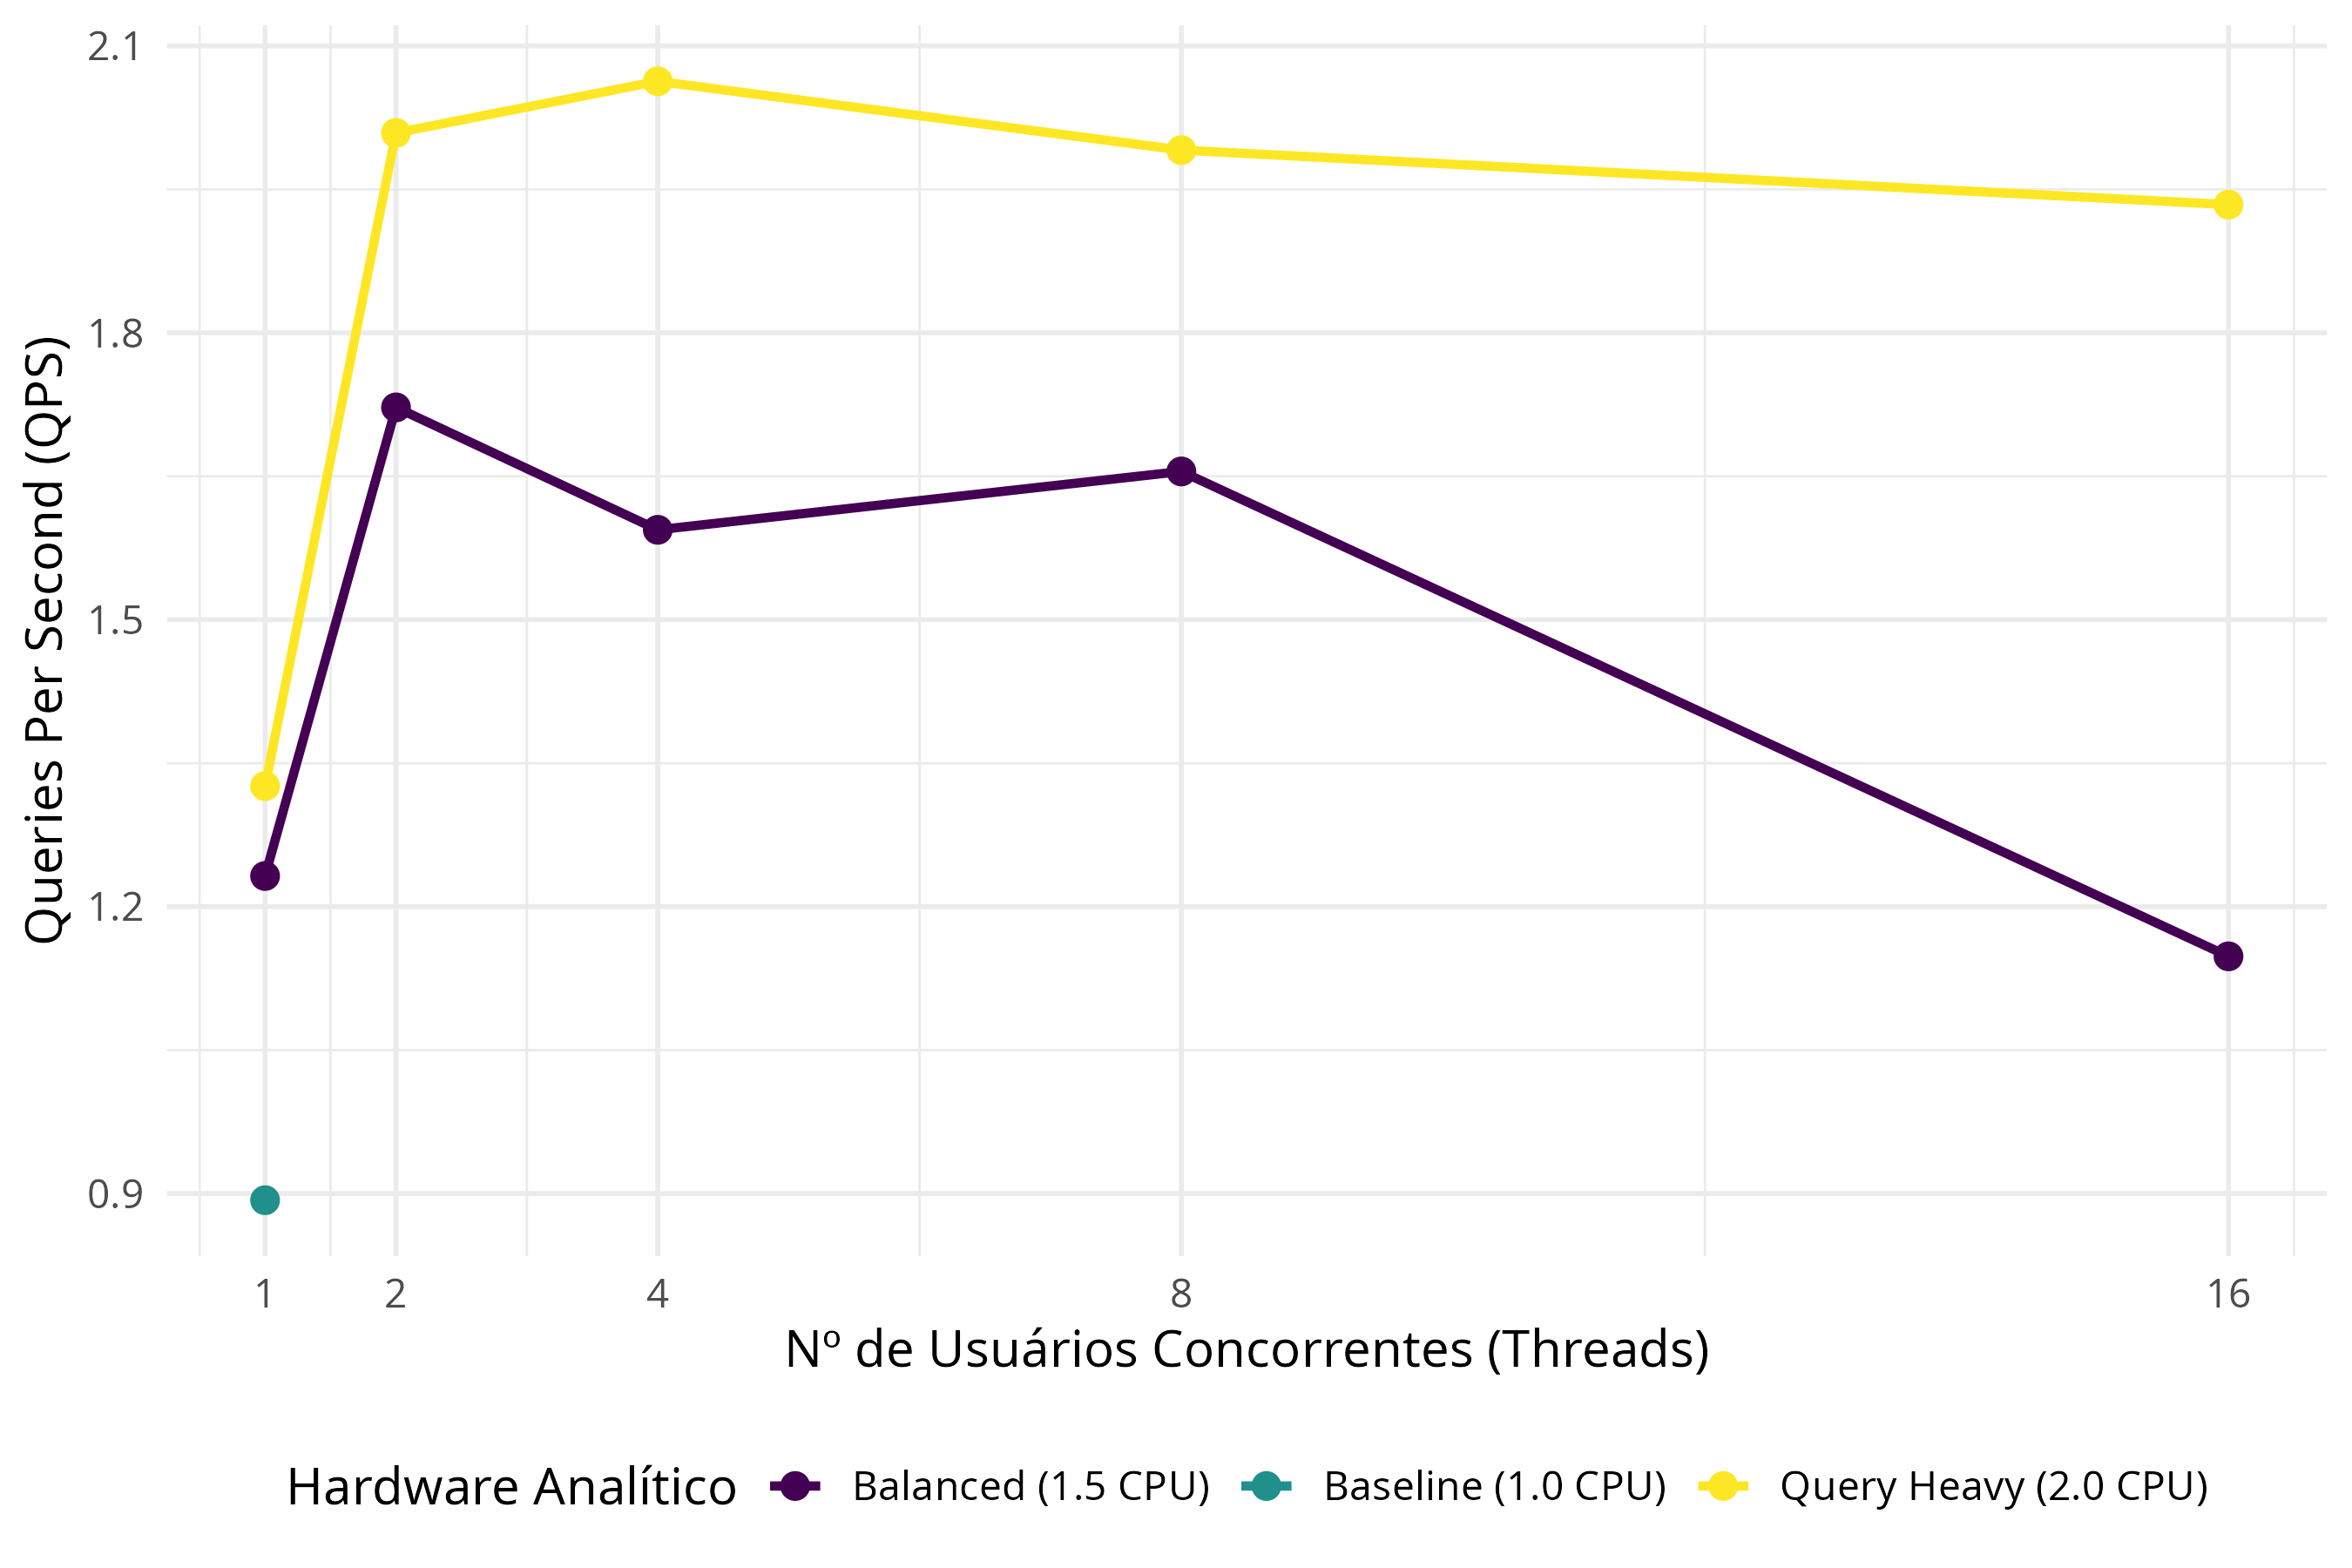
\includegraphics[width=0.47\linewidth]{fig_qps_saturation.png} &
    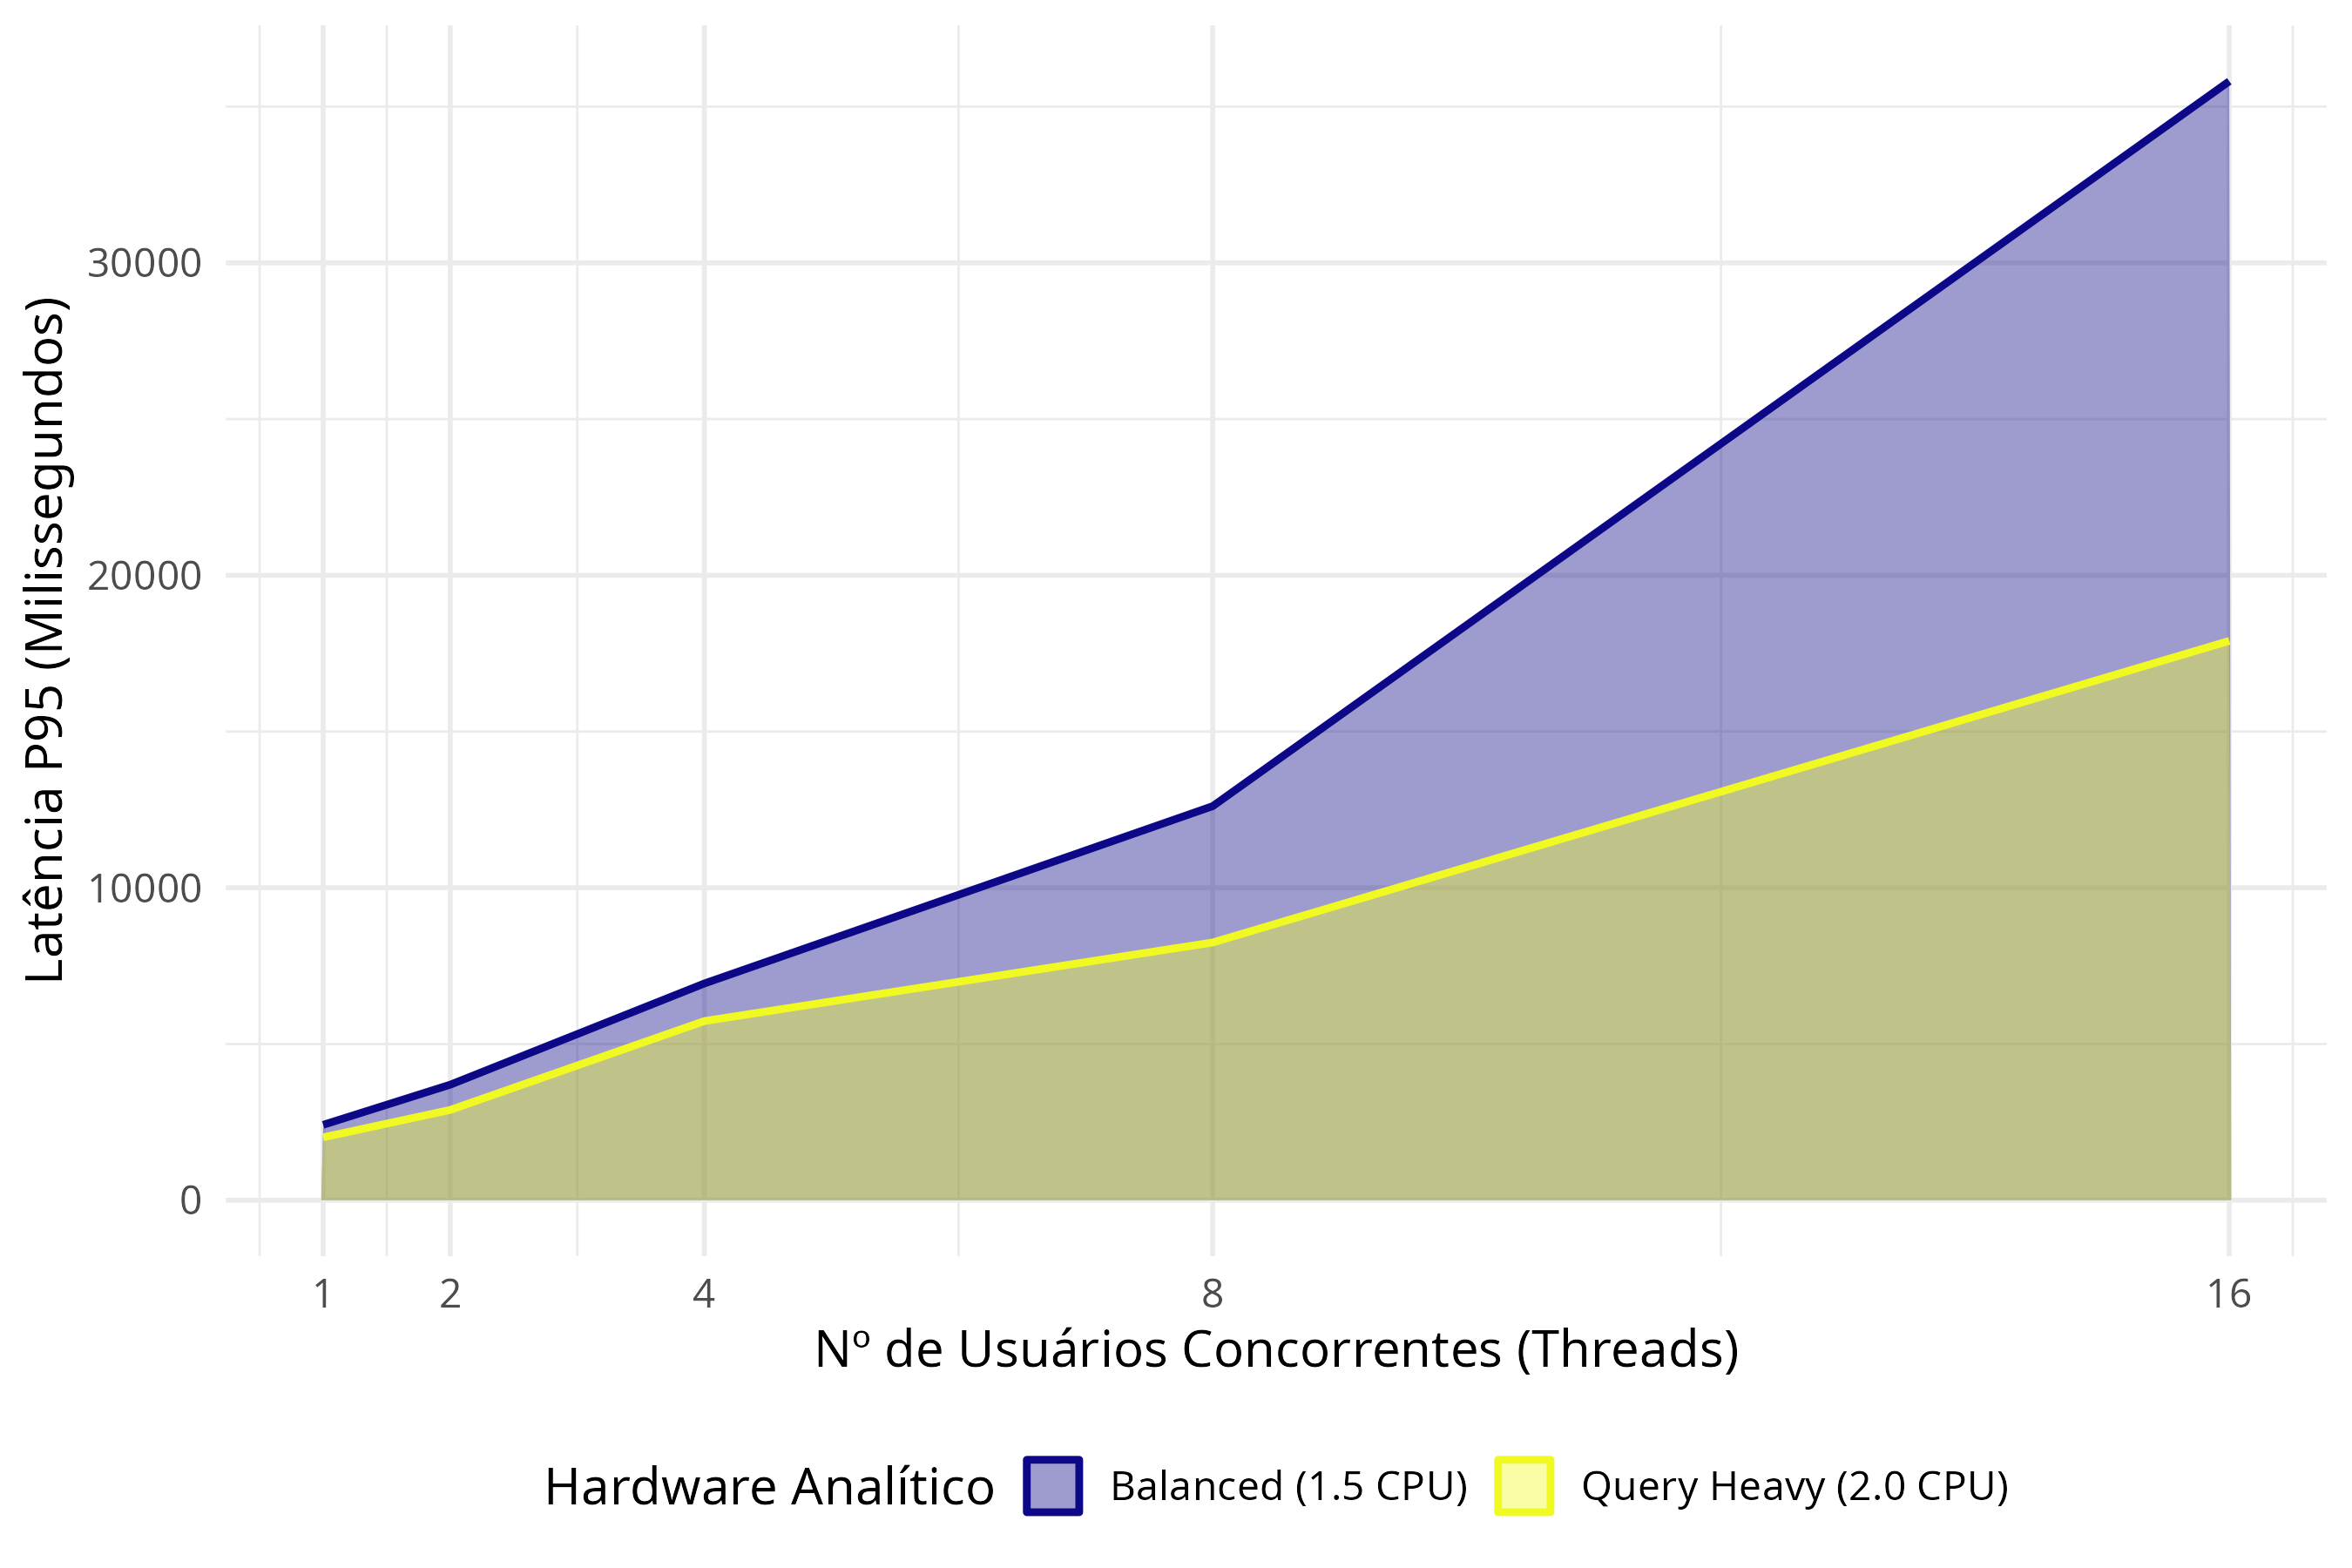
\includegraphics[width=0.47\linewidth]{fig_p95_latency.png} \\
    {\fontsize{13}{16}\selectfont (a) Vazão analítica (QPS) sob estresse} &
    {\fontsize{13}{16}\selectfont (b) Latência P95 por concorrência} \\[0.18cm]
    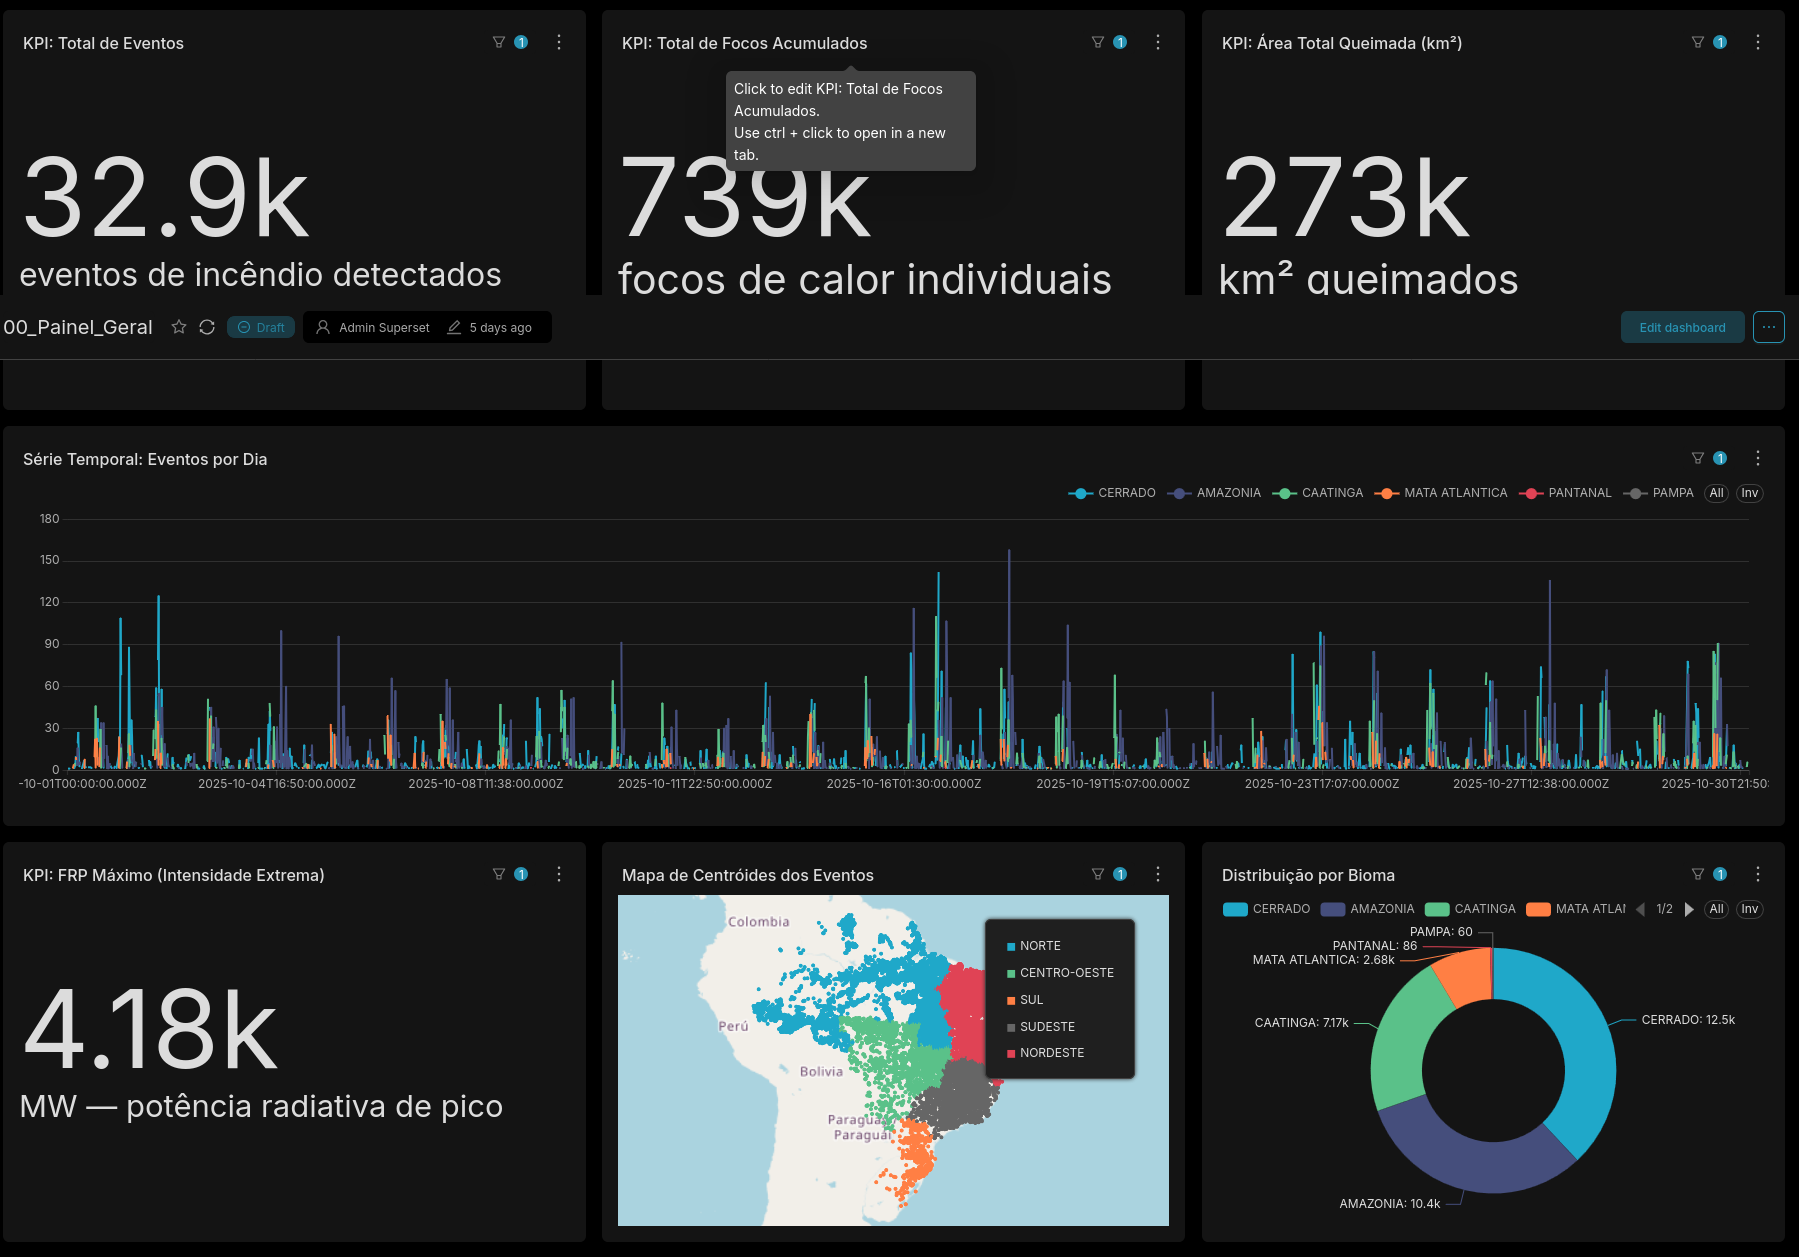
\includegraphics[width=0.47\linewidth]{fig_dashboard_superset.png} &
    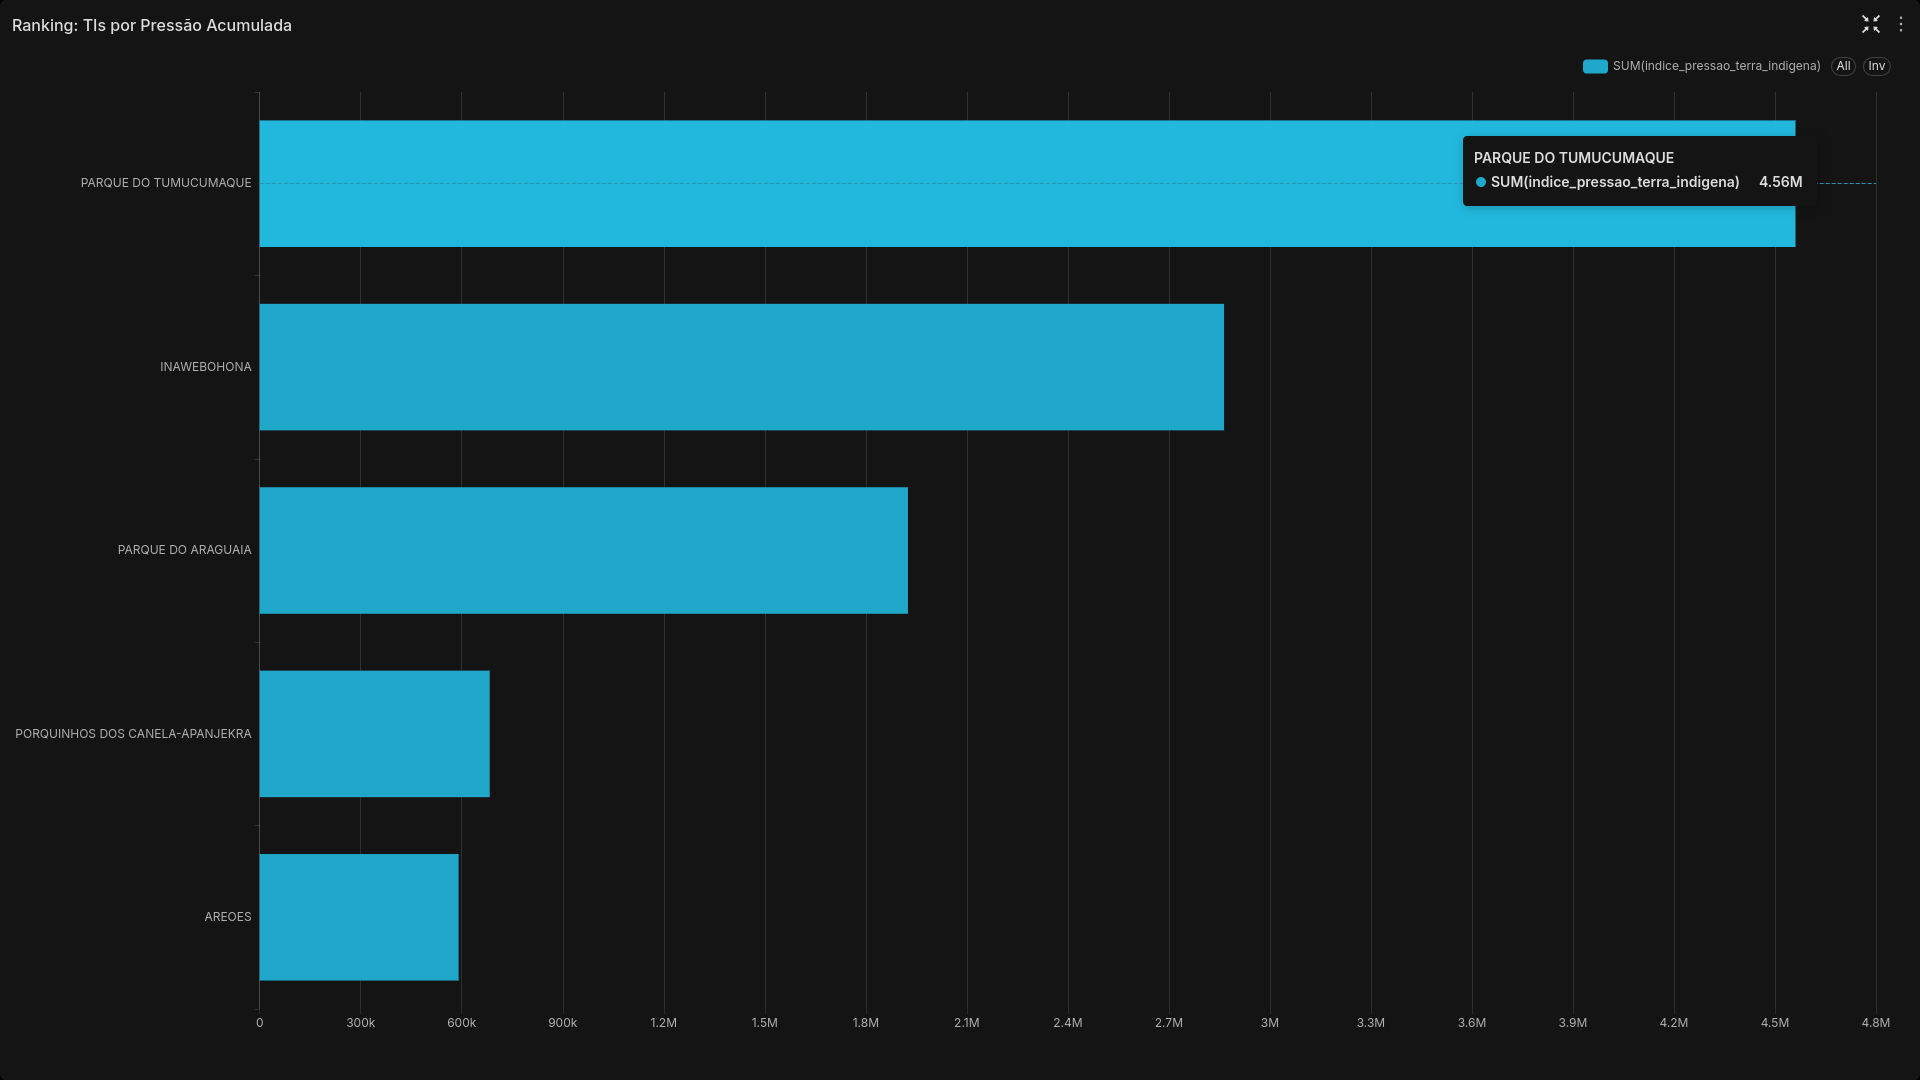
\includegraphics[width=0.47\linewidth]{fig_pressao_indigena.png} \\
    {\fontsize{13}{16}\selectfont (c) Painel tático geral (\textbf{\textit{Superset}})} &
    {\fontsize{13}{16}\selectfont (d) Pressão sobre Terras Indígenas (\textbf{\textit{Bubble Chart}})} \\
\end{tabular}
\vspace{0.08cm}
\captionof{figure}{Evidências empíricas de desempenho analítico e inteligência tática no Brasil.}
\label{fig:grid_resultados}
\end{center}

Na camada de visualização, os painéis operacionais no \textbf{\textit{Apache Superset}} consolidam o fluxo analítico contínuo para subsidiar a tomada de decisão das equipes de emergência e Defesa Civil. A interface gerencial centraliza a contagem de focos ativos e a severidade térmica (FRP), oferecendo filtros dinâmicos por bioma e horizonte temporal para triagens rápidas (Fig. 3c). 

Para além da contagem volumétrica bruta de detecções, a plataforma calcula a pressão contínua exercida sobre áreas protegidas, ponderando a potência radiativa do fogo, o risco meteorológico e o decaimento com a distância: \textbf{\textit{($\boldsymbol{I_{\text{pressão}} = \frac{\text{FRP} \times (1 + \text{risco})}{\max(d_{\text{km}},\, 0{,}1)}}$)}}. A análise sobre os dados de 2025 sugere a existência de um padrão cíclico sazonal de vulnerabilidade térmica, no qual a Terra Indígena Parque do Araguaia (TO) despontou no primeiro lugar em exposição acumulada durante o período de estiagem (Fig. 3d). Essa leitura antecipatória justifica-se pela dinâmica recorrente de avanço do fogo sobre territórios tradicionais, corroborada na prática pelo incêndio de grandes proporções que destruiu dezenas de moradias na Aldeia Canoanã em Formoso do Araguaia (G1 TOCANTINS, 2026).

\vspace{0.20cm}
\section*{CONCLUSÕES}

Os ensaios experimentais sugerem que uma abordagem orientada a eventos pode auxiliar na integração de dados governamentais dispersos sobre queimadas. O patamar de $\sim$2,0 QPS sustentado com 2 vCPU frente à expressiva saturação com 1 vCPU denota que a antecipação de cálculos em memória favorece o tempo de resposta, embora demande dimensionamento cauteloso de hardware sob concorrência. A correlação observada na TI Parque do Araguaia indica o potencial desse modelo para complementar o suporte analítico à Defesa Civil, servindo como camada informativa adicional para o planejamento preventivo em campo.

\vspace{0.20cm}
\section*{AGRADECIMENTOS}

Os autores agradecem à Universidade Federal de Itajubá (UNIFEI) pela infraestrutura física e tecnológica disponibilizada, e ao Conselho Nacional de Desenvolvimento Científico e Tecnológico (CNPq) pela concessão de bolsa de Iniciação Científica e fomento à pesquisa.

\vspace{0.20cm}
\section*{REFERÊNCIAS}

{\fontsize{21}{26}\selectfont
\noindent ENDSLEY, M. R. Toward a theory of situation awareness in dynamic systems. \textbf{Human Factors}, v. 37, n. 1, p. 32-64, 1995.

\vspace{0.18cm}
\noindent G1 TOCANTINS. Incêndio destrói 38 casas em aldeia indígena na Ilha do Bananal. \textbf{G1}, 20 set. 2026.

\vspace{0.18cm}
\noindent INSTITUTO NACIONAL DE PESQUISAS ESPACIAIS (INPE). \textbf{Programa Queimadas: BDQueimadas}. São José dos Campos: INPE, 2026.

\vspace{0.18cm}
\noindent YANG, F. et al. A Fast Column-Store Analytics Database. In: \textbf{ACM SIGMOD International Conference on Management of Data}, 2014. p. 157-168.
\par}


\end{multicols}

\end{document}
